 \documentclass[a4paper, 10pt, conference]{ieeeconf}      % Use this line for a4

%\documentclass[letterpaper, 10 pt, conference]{ieeeconf}  % Comment this line out
                                                          % if you need a4paper
                                                          
\usepackage{FG2019}
\usepackage{multirow}
\newcommand{\minitab}[2][c]{\begin{tabular}{#1}#2\end{tabular}}
\usepackage[acronym]{glossaries}
\usepackage{acronym}
\usepackage{bigstrut}
% symbols for 1/2, etc.
\usepackage{microtype}      % microtypography
\usepackage{amsfonts}       % blackboard math symbols
\usepackage{amssymb}
\usepackage{amsmath}% assumes amsmath package installed
\usepackage[utf8]{inputenc} % allow utf-8 input
\usepackage[T1]{fontenc}    % use 8-bit T1 fonts
% \usepackage{hyperref}       % hyperlinks
\usepackage[colorlinks = true,
            linkcolor = blue,
            urlcolor  = blue,
            citecolor = blue,
            anchorcolor = blue]{hyperref}
            
\usepackage{url}            % simple URL typesetting
\usepackage{mathptmx} % assumes new font selection scheme installed
\usepackage{times} % assumes new font selection scheme installed
\usepackage{lipsum}
% \usepackage{slashbox}
\usepackage{booktabs}       % professional-quality tables
%\usepackage{enumitem}
\usepackage [english]{babel}
\usepackage [autostyle, english = american]{csquotes}
\MakeOuterQuote{"}
\usepackage[font=itshape]{quoting}
\usepackage{lipsum}
% \usepackage{subfig}
%% add
\usepackage{tikz}
\usepackage{graphics}
\usepackage{graphicx}
\usepackage{xcolor}
\usepackage{color, colortbl}
\usepackage{comment}
\usepackage{tabularx, booktabs, ragged2e}
\usepackage{arydshln}
\usepackage{todonotes}
\usepackage{ctable}
\usepackage{multirow}
\usepackage{makecell}

% \usepackage[small]{caption}
% \usepackage{subcaption}
% \usepackage{subfigure} 
\usepackage{sidecap}
\usepackage{wrapfig}
\usepackage[subrefformat=parens,labelformat=parens]{subcaption} %% provides subfigure
\usepackage{caption}
\usepackage{adjustbox}
\usepackage{float}% If comment this, figure moves
\usepackage{geometry}

%\usepackage{algorithm}
%\usepackage{algorithmic}
%\usepackage[]{algorithm2e}
%\usepackage{amssymb}% http://ctan.org/pkg/amssymb
\usepackage{pifont}% http://ctan.org/pkg/pifont


\graphicspath{{images/}} %Setting the graphicspath
\usepackage{bibunits}

\defaultbibliography{bias}
\defaultbibliographystyle{ieee}

\usepackage{mathtools}
\DeclarePairedDelimiter\ceil{\lceil}{\rceil}
\DeclarePairedDelimiter\floor{\lfloor}{\rfloor}


\usepackage{array}
\newcolumntype{x}[1]{>{\centering\arraybackslash\hspace{0pt}}p{#1}}

% \import{sections/}{experimental.tex}
% \import{sections/}{analysis.tex}

% \newcommand{\argmax}{\mathop{\mathrm{argmax}}\limits} 
\newcommand{\argmax}{\mathop{\mathrm{argmax}}\limits} 
\newcommand{\argmin}{\mathop{\mathrm{argmin}}\limits} 

\def\httilde{\mbox{\tt\raisebox{-.5ex}{\symbol{126}}}}

\newcommand{\xmark}{\ding{56}}%
\newcommand{\checkc}{\ding{51}}%

\newcommand{\com}[1]{\textcolor{red}{#1}}
\newcommand{\ie}{\textit{i}.\textit{e}., }
\newcommand{\eg}{\textit{e}.\textit{g}., }
\newcommand*{\etc}{etc.\@\xspace}


\newcommand{\yann}[1]{\todo[color=orange!40]{\rotatebox{90}{YANN: #1}}}
\newcommand{\samson}[1]{\todo[color=blue!40]{\rotatebox{90}{SAMSON: #1}}}
\newcommand{\joe}[1]{\todo[color=purple!40]{\rotatebox{90}{JOE: #1}}}
\newcommand{\bob}[1]{\todo[color=green!40]{\rotatebox{90}{BOB: #1}}}
\newcommand{\gena}[1]{\todo[color=orange!40]{\rotatebox{90}{GENA: #1}}}


\newacronym{m}{M}{\textit{Male}}
\newacronym{f}{F}{\textit{Female}}
\newacronym{a}{A}{\textit{Asian}}
\newacronym{b}{B}{\textit{Black}}
\newacronym{i}{I}{\textit{Indian}}
\newacronym{w}{W}{\textit{White}}
\newacronym{af}{AF}{\textit{Asian}-\textit{Female}}
\newacronym{am}{AM}{\textit{Asian}-\textit{Male}}
\newacronym{bf}{BF}{\textit{Black}-\textit{Female}}
\newacronym{bm}{BM}{\textit{Black}-\textit{Male}}
\newacronym{if}{IF}{\textit{Indian}-\textit{Female}}
\newacronym{im}{IM}{\textit{Indian}-\textit{Male}}
\newacronym{wf}{WF}{\textit{White}-\textit{Female}}
\newacronym{wm}{WM}{\textit{White}-\textit{Male}}

\newacronym{ml}{ML}{machine learning}
\newacronym{fr}{FR}{facial recognition}
\newacronym{fv}{FV}{facial verification}

\newacronym{cnn}{CNN}{convolutional neural network}
\newacronym{nn}{NN}{neural network}
\newacronym{mtcnn}{MTCNN}{\emph{multi-task \gls{cnn}}}

\newacronym{gan}{GAN}{generative adversarial network}
\newacronym{se}{SE}{\emph{Squeeze-and-Excitation}}
\newacronym{d}{$D$}{discriminator}
\newacronym{g}{$G$}{generator}
\newacronym{dbvae}{DB-VAE}{Debiasing Variational Autoencoder}


\newacronym{lut}{LUT}{Look-Up-Table}
\newacronym{soa}{SOTA}{state-of-the-art}

\newacronym{fiw}{FIW}{Families In the Wild}
\newacronym{lfw}{LFW}{Labeled Faces in the Wild}
\newacronym{bfw}{BFW}{Balanced Faces In the Wild}
\newacronym{rfw}{RFW}{Racial Faces in-the-Wild:}
\newacronym{dp}{DemogPairs}{Demographic Pairs}
\newacronym{itwcc}{ITWCC}{Wild Child Celebrity}

\newacronym{fd}{FD}{Face Discrimination}
\newacronym{bb}{BB}{bounding box}

\newacronym{sdm}{SDM}{signal detection model}
\newacronym{roc}{ROC}{receiver operating characteristic}
\newacronym{nmse}{NMSE}{Normalized Mean Square Error}
\newacronym{det}{DET}{Detection Error Trade-off}
\newacronym{tp}{TP}{true-positive}
\newacronym{fp}{FP}{false-positive}

\newacronym{tpir}{TPIR}{true-positive identification rate}
\newacronym{frir}{FRIR}{false-reject identification rate}
\newacronym{fpir}{FRIR}{false-positive identification rate}

\newacronym{fn}{FN}{false-negative}
\newacronym{frr}{FRR}{false-reject rate}
\newacronym{fnr}{FNR}{false-negative rate}

\newacronym{fpr}{FPR}{false-positive rate}
\newacronym{tpr}{TPR}{true-positive rate}


\newacronym{tar}{TAR}{True Acceptance Rate}
\newacronym{far}{FAR}{False Acceptance Rate}
\newacronym{eer}{EER}{Equal Error Rate}

\newacronym{cs}{CS}{Cosine Similiarity}


\newacronym{lime}{LIME}{Local Interpretable Model-Agnostic Explanations}
\newacronym{nas}{NAS}{Neural Architecture Search}
\newacronym{gapf}{GAPF}{Generative Adversarial Privacy and Fairness}
 
                                                          % paper
%\setlist[itemize]{leftmargin=*}
\newcommand{\ra}[1]{\renewcommand{\arraystretch}{#1}}
\newcommand{\mc}[2]{\multicolumn{#1}{c}{#2}}
\definecolor{Gray}{gray}{0.85}
\definecolor{LightCyan}{rgb}{0.88,1,1}

\newcolumntype{a}{>{\columncolor{Gray}}c}
\newcolumntype{b}{>{\columncolor{white}}c}
\renewcommand{\arraystretch}{1.4}
%\newcommand{\xmark}{\ding{53}}%

\newcommand{\highlightb}[1]{%
\colorbox{blue!30}{$\displaystyle#1$}}
\newcommand{\vo}{\vec{o}\@ifnextchar{^}{\,}{}}

\newcommand{\vx}{\vec{x}\@ifnextchar{^}{\,}{}}

\FGfinalcopy % *** Uncomment this line for the final submission
\let\vec\mathbf


% \IEEEoverridecommandlockouts                              % This command is only
                                                          % needed if you want to
                                                          % use the \thanks command
% \overrideIEEEmargins
% See the \addtolength command later in the file to balance the column lengths
% on the last page of the document

% The following packages can be found on http:\\www.ctan.org
%\usepackage{graphics} % for pdf, bitmapped graphics files
%\usepackage{epsfig} % for postscript graphics files



\title{\LARGE \bf\vspace{-10mm}
Face Recognition: Too Bias, or Not Too Bias?
}


%use this in case of several affiliations
\author{\parbox{16cm}{\centering
    {\large Joseph P Robinson$^1$, Gennady Livitz$^2$, Yann Henon$^2$, Can Qin$^1$,\\ Yun Fu$^1$, and Samson Timoner$^2$}\\
    {\normalsize
    \hspace{-.4in}$^{1}$Northeastern University\hspace{.7in} $^{2}$ISM Connect}}
    \thanks{}% <-this % stops a space
}

\begin{document}
%\begin{bibunit}


\def\angle{0}
\def\radius{3}
\def\cyclelist{{"orange","blue","red","green","magenta","cyan"}}
\newcount\cyclecount \cyclecount=-1
\newcount\ind \ind=-1

\ifFGfinal
\thispagestyle{empty}
\pagestyle{empty}
\else
\author{Anonymous FG 2019 submission\\ Paper ID \FGPaperID \\}
\pagestyle{plain}
\fi
\maketitle


%%%%%%%%%%%%%%%%%%%%%%%%%%%%%%%%%%%%%%%%%%%%%%%%%%%%%%%%%%%%%%%%%%%%%%%%%%%%%%%%
\begin{abstract}
We reveal critical insights into problems of bias in state-of-the-art \gls{fr} systems using a novel \gls{bfw} dataset: data balanced for gender and ethnic groups. Classic signal detection theory revealed trends in the underlying score distribution across subgroups. Specifically, we show variations in the optimal scoring threshold varies for face-pairs across different subgroups. Thus, the conventional approach of learning a  global threshold for all pairs resulting in performance gaps among subgroups. By learning subgroup-specific thresholds, we not only mitigate problems in performance gaps but also show a notable boost in the overall performance. Furthermore, we do a human evaluation to measure the bias in humans, which supports the hypothesis that such a bias exists in human perception. To download the \gls{bfw} database, source code, and more, visit \href{https://github.com/visionjo/facerec-bias-bfw}{github.com/visionjo/facerec-bias-bfw}
\end{abstract}
\
%%%%%%%%%%%%%%%%%%%%%%%%%%%%%%%%%%%%%%%%%%%%%%%%%%%%%%%%%%%%%%%%%%%%%%%%%%%%%%%%
\glsresetall
\section{Introduction}
As more of society becomes integrated with \gls{ml}, bias, fairness, and the formalization of \gls{ml} standards are topics of high interest ~\cite{10.1007/978-3-030-13469-3_68, anne2018women, wang2018racial}. One effect of the growing dependency on technology is the increasing concern regarding biased and unfair algorithms.  For instance, \gls{fr} systems can be untrustworthy and racist in some cases~\cite{england2019,snow2018}.
. 

\begin{figure}[t!]
\centering
         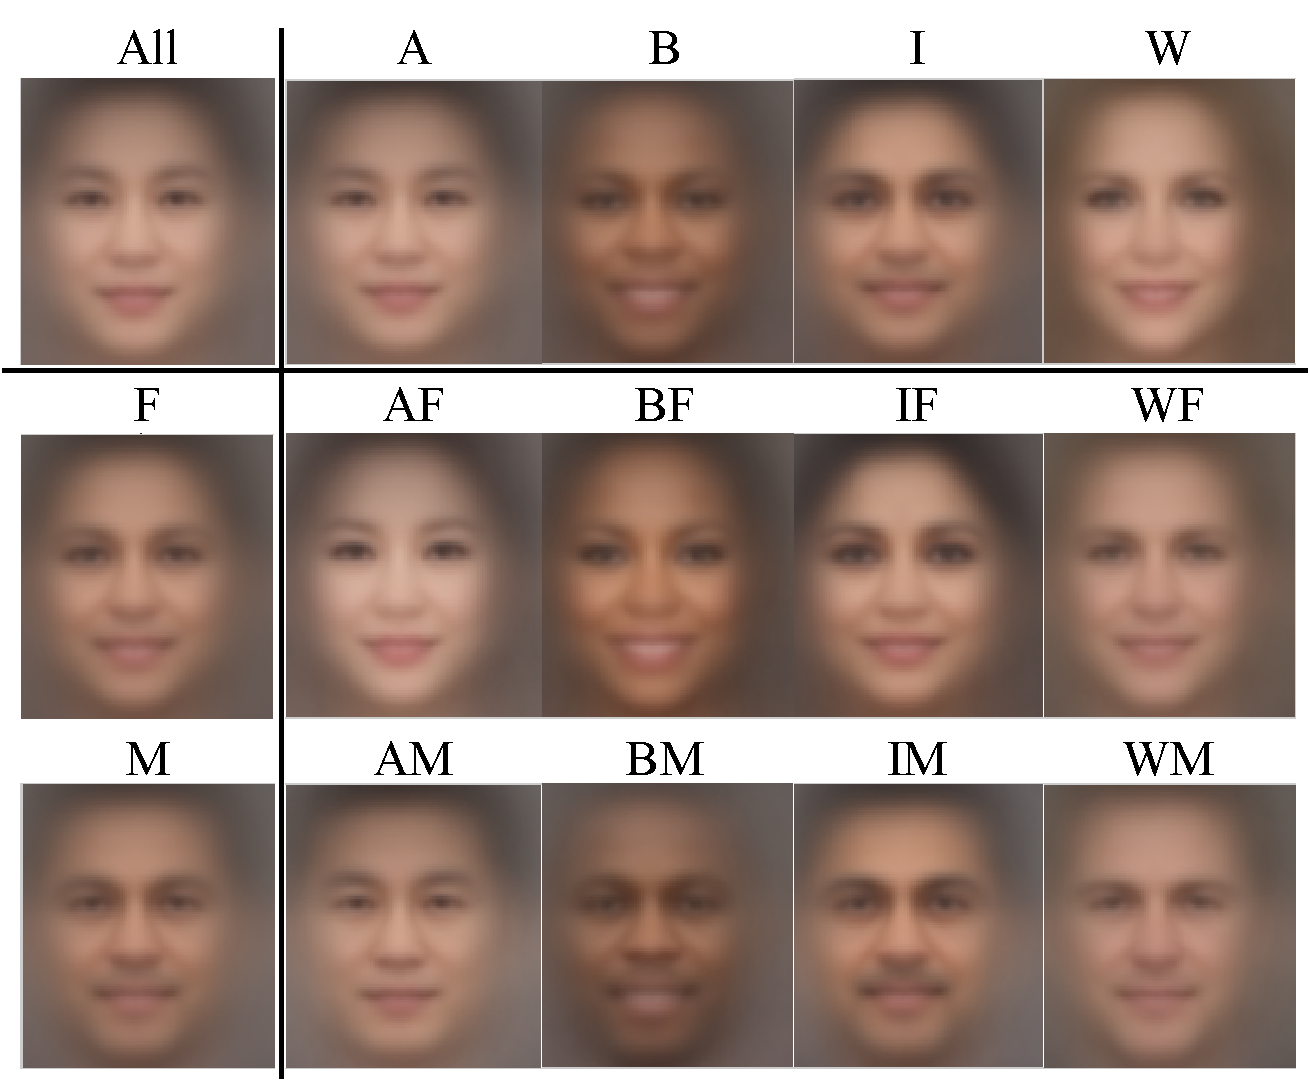
\includegraphics[trim=0in 0.2in 0in 0in,clip,width=.9\linewidth]{images/montage.pdf}  
\caption{\textbf{\gls{bfw}.} The average face of its different subsets: \emph{top-left}: the entire \gls{bfw}; \emph{top-row} per race;  \emph{left-column}: per gender. The others represent the ethnicity and gender of the race and gender, respectfully. Table~\ref{tab:ethnic-splits} defines the acronyms of subgroups.}
\label{fig:avg-faces}
% \vspace{-3pt}
\end{figure}

Typically, \glspl{cnn} are trained on faces identified by a detection system. Specifically, for \gls{fr}, the goal is to project faces to an N-dimensional space with minimal distances between samples of the same identity and maximize the gap separating those that are different. Thus, the overarching goal is to discriminate between subjects with face encodings. We can deploy such a \gls{cnn} to encode faces to compare via a similarity score: genuine pair if the score is high enough; and rejected as an imposter. 

A fixed threshold acts as a decision boundary in similarity score space. Thus, the face features in the same class must satisfy a criterion in the form of a single value~\cite{deng2019arcface, liu2017sphereface, wang2018additive, wang2018cosface}. However, a single, global threshold is a crude measure that leads to \gls{fr} errors. Furthermore, the held-out set used to determine the global threshold tends to share the same distribution with test data, which makes the results skewed in favor of specific demographics that make up a majority in both sets. That skew, the difference in the performance of an algorithm of certain ethnic groups, is our definition of bias. A key question is: \emph{is \gls{fr} too biased, or not?} 


\begin{table*}[t!]
\scriptsize
    \centering
       \caption{\textbf{The proposed \gls{bfw} compared to related datasets.} \gls{bfw} is exactly balanced across ID, gender, and ethnicity (Table~\ref{tab:ethnic-splits}). Compared with \gls{dp}, \gls{bfw} provides more samples per subject and subgroups per set. Also, \gls{bfw} uses a single resource, VGG2. \gls{rfw}, on the other hand, supports a different task (\ie domain adaptation). Furthermore, \gls{rfw} focuses on race-distribution across of pairs, while not considering the distribution of identities. }
    \begin{tabular}{rccccccc}%x{10mm}x{3mm}x{10mm}x{8mm}}%\toprule
    
    \multicolumn{2}{c}{Database} & \multicolumn{3}{c}{Number of}& \multicolumn{3}{c}{Balanced Labels}\\
    \cmidrule(lr){1-2}	\cmidrule(lr){3-5} \cmidrule(lr){6-8}
    Name & Source Data & Faces &  IDs & Subgroups & ID & Ethnicity & Gender\\\midrule
    \gls{dp}~\cite{demogPairs}     & CASIA-W, VGG\&VGG2 & 10,800& 600 & 6 &\checkc& \checkc &\checkc \\
    \gls{rfw}~\cite{wang2018racial}     &  MS-Celeb-1M &$\approx$80,000&$\approx$12,000& 4 & \xmark & \checkc &\xmark \\
    \gls{bfw} (ours) & VGG2 & 20,000 & 800 &8 & \checkc & \checkc &\checkc \\\bottomrule
    \end{tabular}
    \label{tab:compared}
    \vspace{-5mm}
\end{table*}

The adverse effects of a global threshold are two-fold: \textbf{(1)} the mapping produced by a \gls{cnn} is nonuniform. Therefore, distances between pairs of faces in different demographics vary in distribution of similarity scores (Fig~\ref{fig:detection-model}); \textbf{(2)} the evaluation set is imbalanced as well. Particular demographics making up a majority of the population will carry most weight on reported performance ratings. Reported results skew away from common traits to the underrepresented subgroups. Alas, demographics like gender, ethnicity, race, and age are underrepresented in most public datasets. 

Making matters more challenging is that race and ethnicity are loosely defined.  For example, the US Census Bureau allows an individual to self-identify race (\href{https://www.census.gov/mso/www/training/pdf/race-ethnicity-onepager.pdf}{https://www.census.gov}). We define it as a group of people having facial characteristics similar to those found in a region. The result is various types of biases in FR systems in favor of or against particular demographics remain a question.



To address \textbf{(2)}, the lack of a balanced data, we introduce a new benchmark for \gls{fr}, called \gls{bfw} (Table~\ref{tab:compared}, ~\ref{tab:ethnic-splits}). \gls{bfw} serves as a platform to fairly evaluate \gls{fr} systems and enable demographic-specific ratings to be reported. We use \gls{bfw} to gain a deeper understanding of the extent of bias present in facial embeddings extracted from a \gls{soa} \gls{cnn} model. We then suggest a mechanism to counter the biased feature space to mitigate problems of bias with more balanced performance ratings for different demographics, while improving the overall accuracy. Specifically, we propose using an adaptive threshold that varies depending on the characteristics of detected facial attributes (\ie gender and ethnicity, Fig~\ref{fig:avg-faces}). We show an increase in accuracy with a balanced performance for different subgroups of people. Similarly, we show the positive effect of adjusting the similarity threshold based on the facial features of matched faces. Thus, selective use of similarity thresholds in current \gls{soa} \gls{fr} systems provides more intuition in \gls{fr}-based research, while providing a method easily adoptable in practice. 


\begin{table*}[!t]
    \centering
    \caption{\small{\textbf{Database stats and nomenclature, optimal thresholds ($t_o$), and accuracy scores.} \textit{Header:} Subgroup definitions. \textit{Top-row:} Statistics of \gls{bfw}. \textit{Middle-row:} Number of pairs for each partition. \textit{Bottom-row:} Accuracy when applying a global threshold $t_g$, the optimal threshold $t_o$, and accuracy with $t_o$ per subgroup. Columns grouped by race and then further split by gender. Out of millions of pairs, accuracy is inconsistent across subgroups. Furthermore, $F$ tend to perform inferior to that of $M$ (\ie up to 8\%).}}\label{tab:ethnic-splits}
    \scalebox{1}{
     \resizebox{\textwidth}{!}{%
    \begin{tabular}{r c c c c c c c c l}
        \toprule
        & \multicolumn{2}{c}{Asian (A)} & \multicolumn{2}{c}{Black (B)}  & \multicolumn{2}{c}{Indian (I)}& \multicolumn{2}{c}{White (W)}\\
        \cmidrule(l){2-3} \cmidrule(l){4-5} \cmidrule(l){6-7}\cmidrule(l){8-9} % spanning less than the full width of the table - you can add (r) or (l) just before the opening curly bracket to shorten the rule on the left or right side
         & Female (AF) & Male (AM) & BF & BM& IF & IM & WF & WM&Aggregated\\ % Column names row
        \midrule

       \# Faces  &  2,500&  2,500& 2,500 & 2,500& 2,500 & 2,500 & 2,500 & 2,500 &20,000 \\ % row 1
        \# Subjects & 100& 100& 100  & 100  & 100  & 100& 100 &100&800  \\ % row 2
        \# Faces / Subject  & 25 & 25    & 25 & 25 & 25  & 25  &  25 & 25 & 25\\ % row 3
        % \midrule
\specialrule{.01em}{.05em}{.05em}
            \# Positive Pairs &  30,000&  30,000& 30,000 &30,000 & 30,000 &30,000&30,000 & 30,000 &240,000 \\ % row 1
        \# Negative Pairs & 85,135&  85,232& 85,016  & 85,141  & 85,287  & 85,152& 85,223 &85,193&681,379  \\ % row 2

        \# Pairs (Total) & 115,135 & 115,232    &115016 &115,141 & 115287  & 115,152  &  115,223& 115193 & 921,379\\ % row 3
        % \midrule
        \specialrule{.01em}{.05em}{.05em}
        Acc$@t_g$ & 0.876 & 0.944  &0.934 &0.942 &0.922&0.949 &0.916  &0.918&0.925$\pm$0.022 \\
        $t_o$ & 0.235 &  0.274 & 0.267&0.254  &0.299 & 0.295& 0.242 &0.222&0.261\\ % row 4
        Acc$@t_o$ & 0.916 &0.964 &0.955 &0.971 &0.933 &0.958 & 0.969 &0.973 & 0.955 $\pm$ 0.018\\
        \bottomrule
    \end{tabular}}
    \glsunset{af}
    }
    \glsunset{af}
    \glsunset{am}
    \glsunset{bf}
    \glsunset{bm}
    \glsunset{if}
    \glsunset{im}
    \glsunset{wf}
    \glsunset{wm}
    \vspace{-12pt}
\end{table*}




The contributions in this paper are as follows:
\begin{enumerate}
    \item We built a balanced dataset as a proxy to measure verification performance per subgroup.
    \item We analyzed an unwanted bias in scores of face pairs while showing that optimal thresholds determined per subgroup significantly boost and balances performances.
    \item We showed bias causes inconsistencies in ratings across demographics-- the typical use of a global threshold unfavorable. We mitigate the problem via adaptive thresholds.
    \item We conducted human-evaluations to demonstrate bias in human perception.\footnote{NIH-certified, \textit{Protect Humans in Research}, \textcolor{red}{IRB 19-09-08}.}
\end{enumerate}




\section{Background Information}
    \subsection{Bias in \gls{ml}}
        The progress and commercial value of \gls{ml} is exciting; however, the trust of society in \gls{ml} will take time to build due to inherent biases. The exact definitions and implications of bias vary between sources, as do its sources and types. A common theme is that bias hinders performance ratings in ways that skew to a particular sub-population-- the source varies, whether from humans~\cite{windmann1998subconscious}, data and label types~\cite{tommasi2017deeper}, \gls{ml} models~\cite{amini2019uncovering, kim2019learning}, or evaluation protocols~\cite{stock2018convnets}. For instance, a vehicle-detection model might miss cars if training data was mostly trucks. In practice, many \gls{ml} systems learn on biased data, which could be detrimental for society. 


    \subsection{Bias in \gls{fr}}
        Problems of bias in \gls{fr} have been driven by different motivations; therefore, solutions have been posed for different matters. Instances can be in problems of data augmentation~\cite{yin2019feature}, one-shot learning~\cite{ding2018one}, demographic parity and fairness with priority on privacy~\cite{huang2018generative}, domain adaptation~\cite{wang2018racial}, differences in face-based attributes across demographics~\cite{wang2018they}, and even data exploration~\cite{muthukumar2019}. Yin~\etal proposed to augment the feature space of underrepresented classes using other classes with a diverse collection of samples to encourage distributions of underrepresented classes to more closely resemble that of the others~\cite{yin2019feature}. Similarly, others formulated the imbalanced class problem as one-shot learning, where a \gls{gan} was trained to generate face features to augment classes with fewer samples~\cite{ding2018one}. \gls{gapf} was proposed to create fair representations of the data in a quantifiable way, allowing for the finding of a de-correlation scheme from the data without access to its statistics~\cite{huang2018generative}. Wang~\etal defined subgroups at a finer-level (\ie Chinese, Japanese, Korean), and determined the familiarity of faces inter-subgroup~\cite{wang2018they}. Genders have also been used to make subgroups (\eg for analysis of gender-based face encodings~\cite{muthukumar2019}). Most recently,~\cite{wang2018racial} proposed to adapt domains to bridge the bias gap by knowledge transfer, which was supported by a novel data collection, \gls{rfw}. The release of \gls{rfw} occurred after \gls{bfw} was built - although similar in terms of demographics, \gls{rfw} uses faces from MSCeleb~\cite{guo2016ms} for testing, and assumes CASIA-Face~\cite{yi2014learning} and VGG2~\cite{Cao18} were used to train. In contrast, our \gls{bfw} assumes VGG2 as the test set. 
        % As shown in \cite{wang2018racial}, MSCeleb is highly imbalanced, primarily consisting of images of white individuals. 
        % For this, we expect bias from data, for this is the training set. 
        Furthermore, \gls{bfw} balances gender and race: \gls{rfw} splits subgroups by gender and race, while \gls{bfw} has gender, race, or both). 
        % Thus, \gls{rfw} and \gls{bfw} complement one another. % - both add demographic for subjects with faces in renowned, large-scale \gls{fr} datasets.

    
Most similar to us is~\cite{das2018, demogPairs, lopez2019dataset, srinivas2019face} - each were motivated by insufficient paired data for studying bias in \gls{fr}. Then, problems were addressed using labeled data from existing image collections. Specifically, Hupont~\etal curated a set of faces based on racial demographics (\ie \gls{a}, \gls{b}, and \gls{w}) called \gls{dp}~\cite{demogPairs}, while~\cite{srinivas2019face} honed in on adults versus children called \gls{itwcc}. Like the proposed \gls{bfw}, both were built by sampling existing databases, but with the addition of tags for the respective subgroups of interest. Aside from the additional data of \gls{bfw} (\ie added an additional subgroup \gls{i}, along with additional subjects with more faces for all subgroups), we also further split subgroups by gender. Furthermore, we focus on the problem of facial verification and the different levels of sensitivity in cosine similarity scores per subgroup.

    \begin{table*}[t!]
        
        \centering
        \caption{\small{\textbf{\gls{bfw} compared to related datasets.} Our \gls{bfw} is balanced across ID, gender, and ethnicity (Table~\ref{tab:ethnic-splits}). Compared with \gls{dp}, \gls{bfw} provides more samples per subject and subgroups per set, while only using a single resource, VGG2. \gls{rfw}, on the other hand, supports a different task (\ie domain adaptation), and focuses on race-distribution, but not the distribution of identities.}}
        \scriptsize
        \begin{tabular}{rccccccc}%x{10mm}x{3mm}x{10mm}x{8mm}}%\toprule
        
            \multicolumn{2}{c}{Database} & \multicolumn{3}{c}{Number of}& \multicolumn{3}{c}{Balanced Labels}\\
            \cmidrule(lr){1-2}	\cmidrule(lr){3-5} \cmidrule(lr){6-8}
            Name & Source Data & Faces &  IDs & Subgroups & ID & Ethnicity & Gender\\\midrule
            \gls{dp}~\cite{demogPairs}     & CASIA-W~\cite{yi2014learning}, VGG~\cite{schroff2015facenet} \&VGG2~\cite{Cao18} & 10,800& 600 & 6 &\checkc& \checkc &\checkc \\
            \gls{rfw}~\cite{wang2018racial}     &  MS-Celeb-1M &$\approx$80,000&$\approx$12,000& 4 & \xmark & \checkc &\xmark \\
            \gls{bfw} (ours) & VGG2 & 20,000 & 800 &8 & \checkc & \checkc &\checkc \\\bottomrule
        \end{tabular}
        \label{tab:compared}
%            \vspace{-5mm}
    \end{table*}
    
\subsection{Human bias in \gls{ml}}
Bias is not unique to \gls{ml} - humans are also susceptible to a perceived bias. In fact, biases exist across race, gender, and even age~\cite{10.1007/978-3-030-13469-3_68, bar2006, meissner2001, nicholls2018}. Wang~\etal showed machines surpass human performance in discriminating between Japanese, Chinese, or Korean faces by nearly 150\%~\cite{wang2018they}, as humans just pass random (\ie 38.89\% accuracy).

We expect human bias to skew to their own genders and races. For this, we measure the human perception with face pairs of different subgroups (Section~\ref{subsec:human-assessment}). The results concur with~\cite{wang2018they}, as we also recorded overall averages below random ($<$50\%). %The details on settings and number of submissions per demographics are discussed in Section~\ref{}.



%%%%%%%%%%%%%%%%%%%%%%%%%%%%%%%%%%%%%%%%%%%%%%%%%%%%%%%%%%%%%%%%%%%%%%%%%%%%%%%%




%%%%%%%%%%%%%%%%%%%%%%%%%%%%%%%%%%%%%%%%%%%%%%%%%%%%%%%%%%%%%%%%%%%%%%%%%%%%%%%%

\glsunset{if}\glsunset{im}\glsunset{af}\glsunset{am}\glsunset{bf}\glsunset{bm}\glsunset{wf}\glsunset{wm}
\section{The BFW Benchmark and Dataset}


We now discuss the \gls{bfw} dataset, and protocols to evaluate \gls{ml}-based \gls{fr}. We  conclude this section by reviewing the human evaluation conducted as part of this work, to detect bias in humans.

\subsection{The data}
Problems of bias in \gls{fr} motivated the design of \gls{bfw}. The data evenly represent various subgroups partitioned by demographics. Inspired by \gls{dp}~\cite{demogPairs}, the specification of \gls{bfw} follows in suit. \gls{bfw} includes additional subgroups (\ie \gls{if} and \gls{im}), an increased in the number subjects per subgroup, with many more pairs (Table~\ref{tab:ethnic-splits}). 




\vspace{1mm}
\noindent\textbf{Compiling subject list.} 
 All subjects were sampled from VGG2~\cite{Cao18}. Thus, unlike others that depend on multiple sources, \gls{bfw} has less potential conflicts in train/test overlap for existing models. We used pre-trained ethnicity~\cite{ambekar2009name} and gender~\cite{levi2015age} classifiers to find candidates for the different subgroups.



\vspace{1mm}
\noindent\textbf{Detecting faces.} Faces were detected using \gls{mtcnn}~\cite{zhang2016joint}.\footnote{\href{https://github.com/polarisZhao/mtcnn-pytorch}{https://github.com/polarisZhao/mtcnn-pytorch}} Then, assigned into one of two sets. Faces within detected bounding box (BB) regions extended out 130\% in each direction, with zero-padding as the boundary condition made-up one set. The second set were faces aligned and cropped for Arcface~\cite{deng2019arcface} (see the next step). Also, coordinates of the BB and the five landmarks per MTCNN were stored as part of the static, raw data. Samples with multiple face detections had the BB area times the confidence score of the MTCNN to determine the instance most likely to be the face, with others set aside and labeled \textit{miss-detection}. 

\begin{figure}[!t] 
	\centering    
 \glsunset{fpr}
  \glsunset{fnr}
	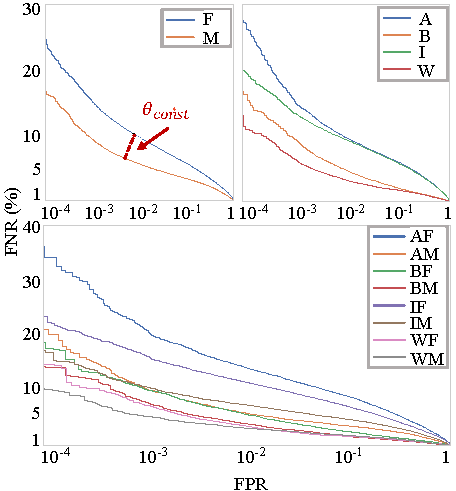
\includegraphics[width=\linewidth]{figures/detcurve-improved.pdf}
		\caption{\textbf{\gls{det} curves.} \emph{Top-left}: per gender. \emph{Top-right}: per ethnicity. \emph{Bottom}: per subgroup (\ie combined). A dashed lined shows a difference by about 2$\times$ in \gls{fpr} for the same threshold $\theta_{const}$. \gls{fnr} is the number of match errors, so closer a curve is to the bottom better.}
		\glsreset{det}\glsreset{fpr}
\label{fig:detcurves} 
\end{figure} 

\vspace{1mm}
\noindent\textbf{Validating labels.} 
Faces of \gls{bfw} were encoded using the original implementation of the \gls{soa} Arcface~\cite{deng2019arcface}. A matrix of cosine similarity scores was then generated for each subject, and removed samples (\ie rows) with median scores below threshold $\theta=0.2$. Mathematically, the $j^{th}$ subject with $N_j$ faces is removed if the ordinal rank of its score $n = \frac{P\times N}{100}\geq\theta$, with the percentile $P=50$, $\theta=0.2$ set manually, and an ordered list of scores. This allowed us to quickly prune \gls{fp} face detections. Following~\cite{robinson2016families, robinson2018visual}, we built a JAVA tool to visually validate the remaining faces. The faces were first ordered from most-to-least confidence, with confidence set as the average score, and then displayed as image icons on top toggling buttons arranged as a grid in a sliding pane window. Labeling then consisted of going subject-by-subject and flagging faces of \emph{imposters}. 


\vspace{1mm}
\noindent\textbf{Sampling faces and creating folds.} We created lists of pairs in five-folds with subjects split evenly per subject and without overlap across folds. Furthermore, balance in the number of faces per was obtained by sampling twenty-five faces at random from each. Next, we generated a list of all face pairs per subject, resulting in $\sum_{l=1}^{L}\sum_{k=1}^{K_d} {N_k \choose 2}$ positive pairs, where the number of faces of all $K_l$ subjects $N_k=25$  for each of the $L$ subgroups (Table~\ref{tab:ethnic-splits}). Next, we assigned subjects to a fold. To preserve balance across folds, we sorted subjects by the number of pairs and then started assigning to alternating folds from the one with the most samples. Note, this left no overlap in identity between folds. Later, a negative set from samples within the same subgroup randomly matched until the count met that of the positive. Finally, we doubled the total count with negative pairs from across subgroups but in the same fold.
\begin{figure}[t!] 
	\glsunset{fpr}
	\centering
	\centering
	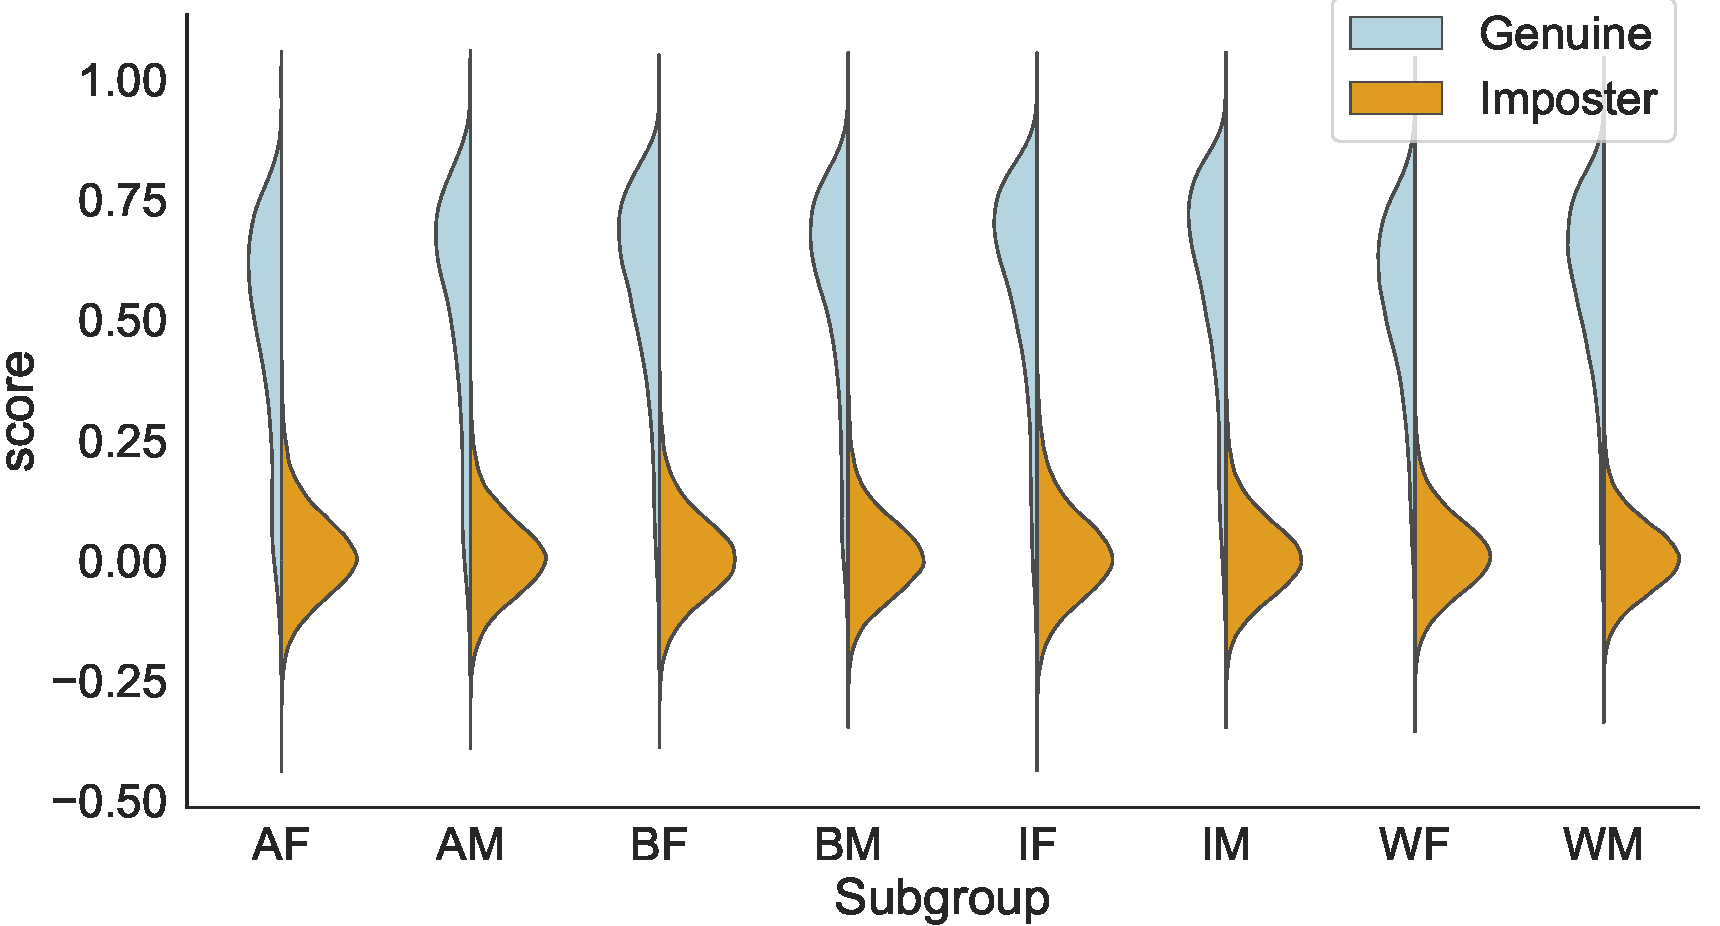
\includegraphics[width=1\linewidth]{figures/violinplots.pdf}
		\caption{\textbf{\Gls{sdm} across subgroups.} The scores for \emph{imposters} have medians about 0.3 but with variation in upper percentiles, while \emph{genuine} pairs vary in both (\eg \gls{af} has more area of overlap). A varying threshold varying across different subgroups yields a constant \gls{fpr}.} \label{fig:detection-model} 
		
\end{figure} 


\vspace{-5pt}
\subsection{Problem formulation}\label{subsec:pf} 
% \gls{lfw}~\cite{LFWTech}, a commonly used benchmark for ~\gls{fr}, reserves specific train-test face-pair lists. 
\Gls{fv} is the special case of the two-class (\ie boolean) classification. Hence, pairs are labeled as the ``same'' or ``different'' \textit{genuine} pairs (\ie \textit{match}) or \textit{imposter} (\ie \textit{mismatch}), respectfully. This formulation (\ie \gls{fv}) is highly practical for applications like access control, re-identification, and surveillance. Typically, training a separate model for each unique subjects is infeasible. Firstly, the computational costs compound as the number of subjects increase.  Secondly, such a scheme would require model retraining each time a new person is added. Instead, we train models to encode facial images in a feature space that captures the uniqueness of a face, to then determine the outcome based on the output of a scoring (or distance) function. Formally put:
\begin{equation}\label{eg:matcher}
    f_{boolean}(\vec{x}_i, \vec{x}_j) = d(\vec{x}_i, \vec{x}_j) \leq \theta
\end{equation}

where $f_{boolean}$ is the \textit{matcher} of the feature vector $\vec{x}$ for the $i^{th}$ and $j^{th}$ sample~\cite{LFWTech}.

Cosine similarity is used as the \emph{matcher} in Eq~\ref{eg:matcher} the closeness of $i^{th}$ and $j^{th}$ features, \ie
$
s_l= \frac{f_i\cdot f_j}{||f_i||_2||f_j||_2}
$ is the closeness of the $l^{th}$ pair. 


\subsection{Human Assessment}\label{subsec:human-assessment}
We evaluated human on face pairs focusing on two racial groups: Chinese and Caucasians. To focus on the experiment, we honed-in on two groups, white Americans (W) and Chinese from China (C). The purpose was to the minimize variability by only analyzing the subsets of the broader groups of whites and Asians. 

Samples were collected by recruiting subjects from multiple sources (\eg social media, email lists, and family/friends)-- a total of 120 participants were sampled at random from all the submissions that were (1) complete and (2) from a W or C participant. Specifically, there were 60 W and 60 C, both with \gls{m} and \gls{f} split evenly. A total of 50 face pairs of non-famous ``look-alikes'' were collected from the internet, with 20 ({\emph WA}) and 20 ({\emph C}) pairs (male and female split evenly). The other 10 pairs are of others (\eg Hispanic/ Latino, Japanese, African). Survey was created, distributed, and recorded via \href{https://paperform.co}{PaperForm}. 



%%%%%%%%%%%%%%%%%%%%%%%%%%%%%%%%%%%%%%%%%%%%%%%%%%%%%%%%%%%%%%%%%%%%%%%%%%%%%%%%


\begin{figure}[t!]
	\centering    
	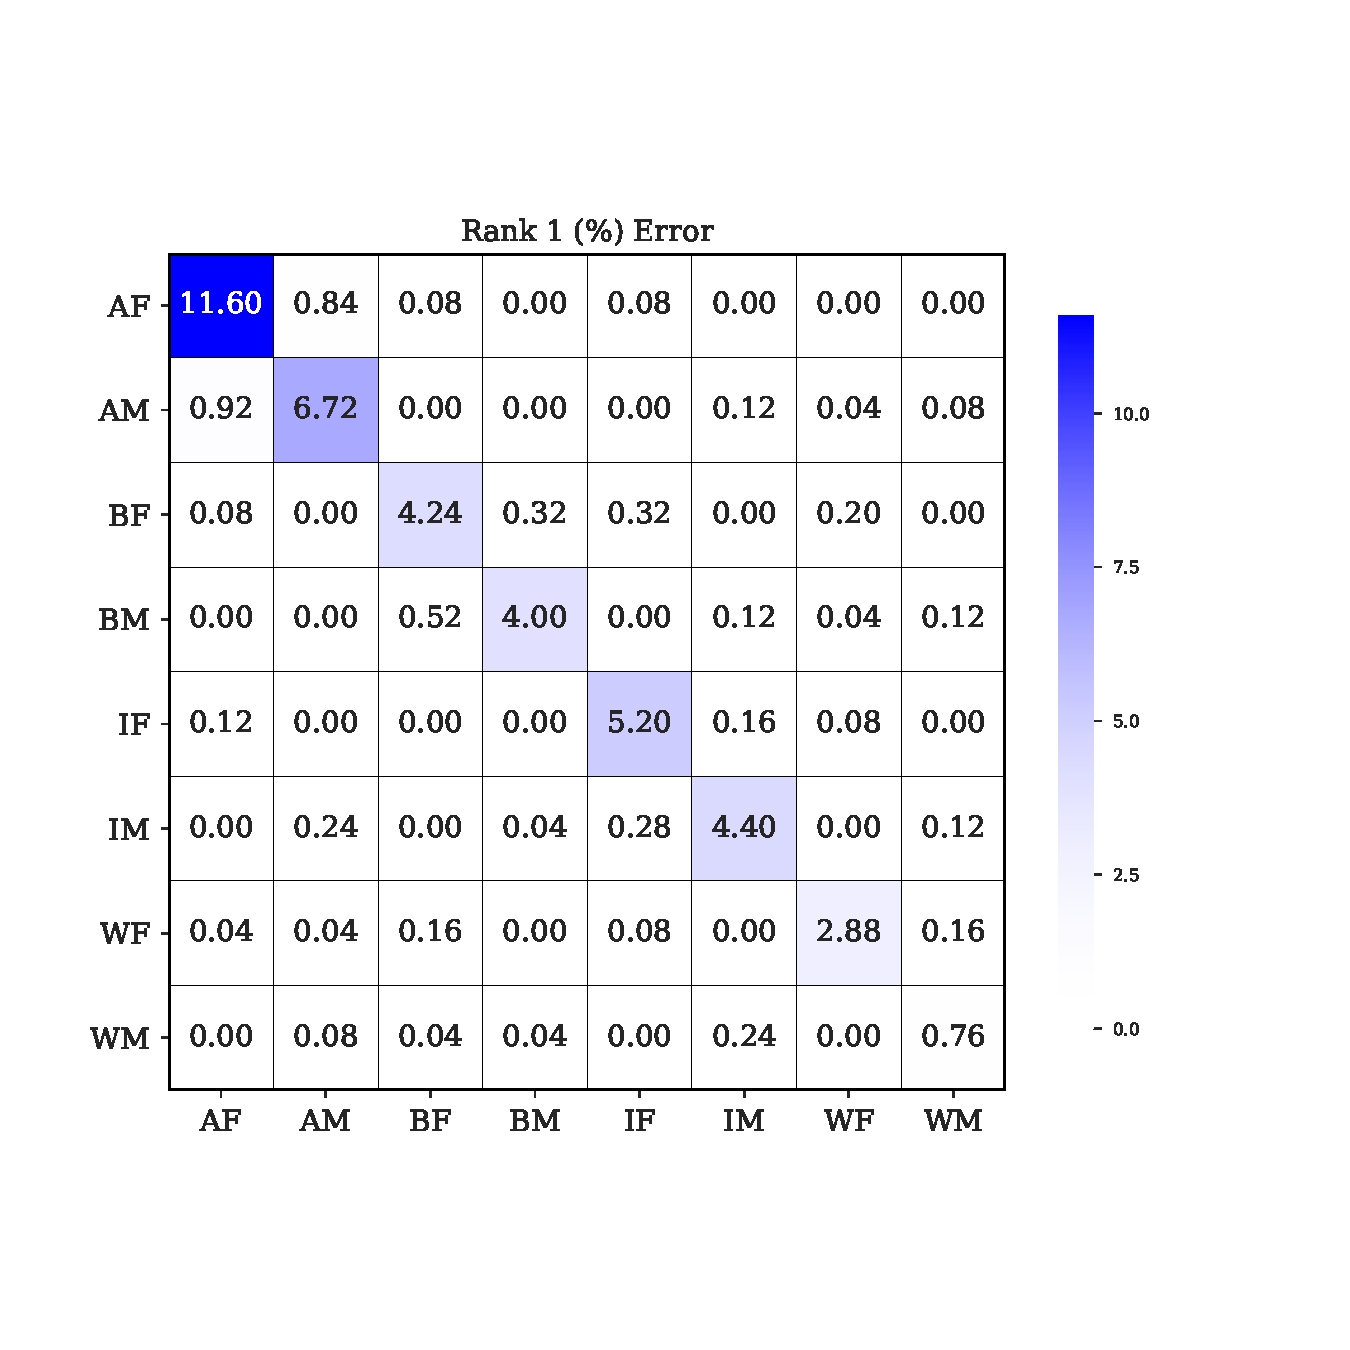
\includegraphics[width=\linewidth]{images/confusion.pdf}
		\caption{\small{\textbf{Confusion matrix.} Percent error (Rank 1) for all faces of \gls{bfw} queried against all others. Notice errors concentrate within a subgroup, consistent with the \gls{sdm} in Fig.~\ref{fig:detection-model} (\ie \gls{af} show worst performance, and is mostly confused with faces of the same demographic). This plot is evidence that while race/ethnicity may be challenging to define, the subgroups are meaningful.}}
		\label{fig:confusion} 
		\vspace{-5mm}
\end{figure} 

\section{Results and Analysis}
An {\em off-the-shelf} \gls{cnn} was used throughout to control the model across all experiments. For this, Sphereface~\cite{liu2017sphereface} trained on CASIA-Web~\cite{yi2014learning}, and evaluated on \gls{lfw}~\cite{LFWTech} (\%99.22 accuracy), encoded all of the faces.\footnote{\href{https://github.com/clcarwin/sphereface_pytorch}{https://github.com/clcarwin/sphereface_pytorch}} Following~\cite{liu2017sphereface}, upon applying an affine transformation to align faces according to pre-defined eye locations, each face got fed through the network twice, the original and horizontally flipped. The two features were fused by concatenation.

Additional \gls{cnn}-based models demonstrate the same phenomena: proportional to the overall model performance, exact in which the ordering subgroups in sensitivity in scores space (Appendix~\ref{app:sec:other:models}).
% Specifically, we analyze three \glspl{cnn} variants: we encode faces using VGG-16~\cite{simonyan2014very},  50-layer residual network (\ie ResNet-50)~\cite{he2016deep}, and \gls{senet} (\ie SENet-50)~\cite{hu2018squeeze}, with results of only the latter (\ie the best performing \gls{senet}) model used throughout the main paper. Results for the other two, alongside \gls{senet} for comparison, are in the Supplemental Material.


\glsunset{am}\glsunset{af}\glsunset{bm}\glsunset{bf}\glsunset{im}\glsunset{if}\glsunset{wm}\glsunset{wf}




% \vspace{-2pt}
\subsection{Score Analysis}
Fig.~\ref{fig:detection-model} shows score distributions for faces of the same identity (\ie \emph{Genuine}) and different (\ie \emph{Imposter}), with \gls{sdm}s split by subgroup. Observe that scores of imposters  approximately distribute about a peak of zero independent of subgroup, with slightly different standard deviation. Observe that the broadness in score distribution of the \emph{genuine} pairs varies across subgroups. Asian Fem
Fig.~\ref{fig:confusion} shows the confusion matrix of the subgroups. A vast majority of errors occurs in intra-subgroup. It is interesting to note that while the definition of  each group  based on ethnicity and race may not be crisply defined, the confusion matrix indicates that in practice the \gls{cnn} finds that the groups are effectively separate. The categories are, therefore, meaningful in the context of \gls{fr}.


\subsection{\gls{det} analysis}
\glsunset{m}
\glsunset{f}

\gls{det} curves averaged across 5-folds show per-subgroup trade-offs (Fig.~\ref{fig:detcurves}). Note that \gls{m} perform better than \gls{f}, precisely as one would expect from the tails of score-distributions for \emph{genuine} pairs (Fig.~\ref{fig:detection-model}). \Gls{af} and \gls{if} perform the worst.


 
\begin{table}[t!]
\glsunset{tar}
\glsunset{far}
\caption{\small{\textbf{\gls{tar} at intervals of \gls{far}}. For each subgroup, and overall average \gls{far}, listed are the \gls{tar} scores for a global threshold (top) and the proposed category-based threshold (bottom). Higher is better. The proposed shows improvement in all cases.}}\label{tab:ethnicy-far} 
\begin{center}
\begin{tabular}{l c c c c c}
     \gls{far} & 0.3 & 0.1 & 0.01 & 0.001 & 0.0001\\\midrule
    \multirow{2}{.1mm}{\textbf{\gls{af}}} &0.990 & 0.867 & 0.516 & 0.470 & 0.465\\[-4pt]
        &1.000 & 0.882 & 0.524 & 0.478 & 0.474\\[-1pt]
    \multirow{2}{3mm}{\textbf{\gls{am}}} &0.994 & 0.883 & 0.529 & 0.482 & 0.477\\[-4pt]
        &1.000 & 0.890 & 0.533 & 0.486 & 0.482\\[-1pt]
    \multirow{2}{3mm}{\textbf{\gls{bf}}} &0.991 & 0.870 & 0.524 & 0.479 & 0.473\\[-4pt]
        &1.000 & 0.879 & 0.530 & 0.484 & 0.480\\[-1pt]
    \multirow{2}{3mm}{\textbf{\gls{bm}}} &0.992 & 0.881 & 0.526 & 0.480 & 0.474\\[-4pt]
        &1.000 & 0.891 & 0.532 & 0.485 & 0.480\\[-1pt]
    \multirow{2}{3mm}{\textbf{\gls{if}}} &0.996 & 0.881 & 0.532 & 0.486 & 0.481\\[-4pt]
        &1.000 & 0.884 & 0.534 & 0.488 & 0.484\\[-1pt]
    \multirow{2}{3mm}{\textbf{\gls{im}}} &0.997 & 0.895 & 0.533 & 0.485 & 0.479\\[-4pt]
        &1.000 & 0.898 & 0.535 & 0.486 & 0.481\\[-1pt]
    \multirow{2}{3mm}{\textbf{\gls{wf}}} &0.988 & 0.878 & 0.517 & 0.469 & 0.464\\[-4pt]
        &1.000 & 0.894 & 0.526 & 0.478 & 0.474\\[-1pt]
    \multirow{2}{3mm}{\textbf{\gls{wm}}} &0.989 & 0.896 & 0.527 & 0.476 & 0.470\\[-4pt]
        &1.000 & 0.910 & 0.535 & 0.483 & 0.478\\[-1pt]
    \midrule
    \multirow{2}{3mm}{\textbf{Avg.}} &0.992 & 0.881 & 0.526 & 0.478 & 0.474\\[-4pt]
        &1.000 & 0.891 & 0.531 & 0.483 & 0.479\\[-10pt]
\end{tabular}
\end{center}
\glsreset{tar}
\glsreset{far}
\end{table}


The gender-based \gls{det} curve shows that there are different performances for \gls{m} and \gls{f} at a fixed threshold (dashed-line). Similar effects exist for the other curves as well (lines omitted to declutter). Many \gls{fr} applications, systems are operated at the highest \gls{fpr} allowed, so the line of constant threshold indicates that a single threshold produced at different operating points (\ie \gls{fpr}) \gls{m} and \gls{f}, which is undesirable.  The difference in \gls{fpr} is approximately a factor of 2-- quite large indeed. If this kind of difference is common in industry, one would expect a factor of 3 more false positives to be reported based on one subgroup than another, which has a strong potential to be the cause of media articles reporting bias in 
\gls{fr}~\cite{england2019,snow2018}.


\subsection{Verification threshold} \label{subsec:analysis:verification}
We seek to reduce the bias between subgroups. Such that an operating point (\ie \gls{fpr}) is constant across subgroups. To accomplish that, we used a per subgroup threshold. In \gls{fv}, we consider one image as the query and all others as test. For this, the ethnicity of the query image is assumed. We can then examine the \gls{det} curves and pick the best threshold per subgroup for a certain \gls{fpr}.

We evaluated \gls{tar} for specific \gls{far} values. As described in Section~\ref{subsec:pf}, the verification experiments were 5-fold, with no overlap in subject ID between folds. Results reported are averaged across folds in all cases and are shown in Table~\ref{tab:ethnicy-far}. For each subgroup, the \gls{tar} of using a global-threshold is reported (upper row), as well as using the optimal per subgroup threshold (lower row). 

Even for lower \gls{far}, there are notable improvements, often of the order of 1\%, which can be challenging to achieve when \gls{far} is near $\geq$90\%. More importantly, each subgroup has the desired \gls{fpr}, so that substantial differences in \gls{fpr} will remain unfounded. We further experimented using ethnicity estimators and using the ethnicity of both query and test image, which yielded similar results to those reported here (results not shown).

\begin{figure}[t!] 
	\centering    
	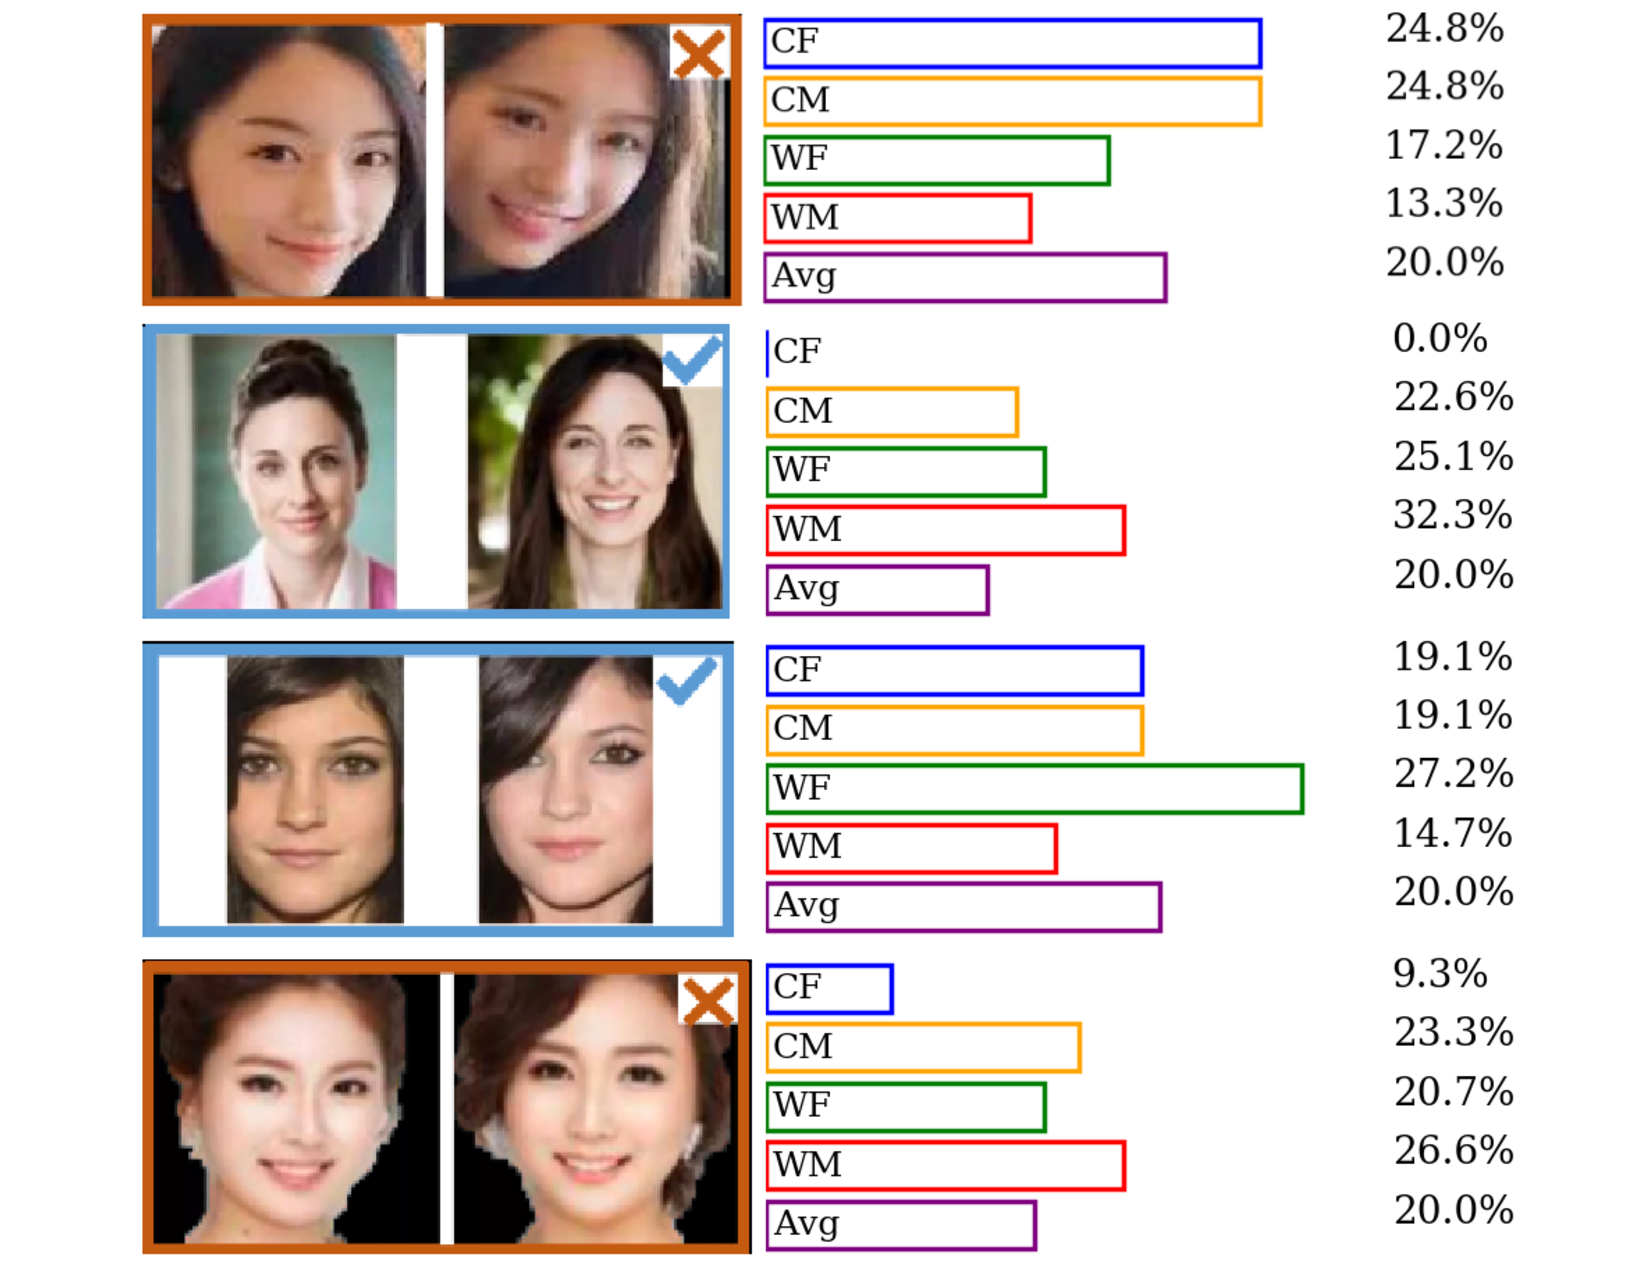
\includegraphics[trim=0in 0.0in 0in 0in,clip, width=\linewidth] {images/human_eval.pdf}
		\caption{\small{\textbf{Qualitative results of human assessment.} $\checkmark$ for \emph{match}; $\times$ for \emph{non-match}, which scores plotted next to each. Humans tend to be more successful at recognizing their own subgroup, with few exceptions (bottom). }}
		% (\eg bottom row). } Result summary in Table~\ref{tab:human-eval}.
		\label{fig:human-eval} 
		\vspace{-5mm}
\end{figure} 

% \vspace{-5pt}
\subsection{Human evaluation}
 Quantitative and qualitative results are in Table~\ref{tab:humsn-eval-results} and Fig.~\ref{fig:human-eval}, respectfully. One might expect that the most exposure to others would be within the same subgroup, and, therefore, would be best at labeling their own. Secondarily, they would be best at labeling images of the same ethnicity, but opposite gender. Our findings concur. Each subgroup is best at labeling their type, and then second best at labeling the same ethnicity but opposite sex. Interestingly, each group of images is best tagged by the corresponding subgroup, with the second-to-best having the same ethnicity and opposite gender. On average, subgroups are comparable at labeling images. 






%%%%%%%%%%%%%%%%%%%%%%%%%%%%%%%%%%%%%%%%%%%%%%%%%%%%%%%%%%%%%%%%%%%%%%%%%%%%%%%%
\begin{table}[t!]
\begin{center}
    \caption{\small{\textbf{Quantitative of human assessment.} Different human subgroups listed per row. Each column is the subgroup labeled. Note that each people are best within their subgroup, and second-best within the same subgroup but different gender. CF shows the least variation, but with the lowest accuracy. CM shows the best accuracy, but second to \gls{wm} in deviation from the mean. Thus, scores for males vary more than females.}}
    \label{tab:humsn-eval-results} 
     \vspace{-2mm}

\footnotesize
\scalebox{0.9}{
\begin{tabular}{l c c c c c}
        &  CF  &      CM     &   WF     &   WM     &  Avg\\\midrule
        CF &  \textbf{0.529}&  0.480&0.438&0.447 &0.474$\pm$0.041 \\
        CM & 0.456 & \textbf{0.504}  & 0.444 &0.362 &0.441$\pm$0.059 \\
        WF & 0.447 &0.438 &  \textbf{0.573}& 0.480 & 0.485$\pm$0.062 \\
        WM & 0.301&0.474 &  0.453 & \textbf{0.561} & 0.447$\pm$0.108 \\\midrule
        Avg &  0.433& 0.474&0.477 &0.463 &0.462$\pm$0.020\\
 \end{tabular}}
 \end{center}
 \vspace{-6mm}
\end{table} 

\glsresetall
\vspace{-1mm}
\section{CONCLUSION}
We introduce a new data set \gls{bfw} with eight subgroups balanced across gender and ethnicity. With this, and upon highlighting the challenges and shortcomings of grouping subjects as a single subset, we provide evidence that forming subgroups is meaningful, as the \gls{fr} algorithm rarely makes mistakes across subgroups. We trained Arc-Face net on MSCeleb, expecting that the results would suffer from bias because of the imbalanced train-set. Once established that the results do suffer from problems of bias, we observed that the same threshold across ethnic and gender subgroups leads to differences in the \gls{fpr} up to a factor of two, which is seemingly the cause of the frenzy about bias in \gls{fr} in main-stream media. Furthermore, we ameliorate these differences with a per-subgroup threshold, leveling out \gls{fpr}, and achieving a higher \gls{tpr}. We hypothesized that most humans grown amongst more than their own demographic and, therefore, effectively learn from imbalanced datasets-- a human evaluation validated that humans are biased, as most recognized their personal demographic best. The focused research findings presented here, along with the public database included, are extendable in vast ways. Thus, we see this as the slither to a much larger problem of bias in ML.

\vspace{-3mm}
\bibliographystyle{ieee}
\bibliography{bias}

% \putbib
% \end{bibunit}
\begin{bibunit}
%
\newpage
\onecolumn
% \begin{minipage*}[\linewidth]{width of the minipage}
\renewcommand{\thesection}{\alph{section}}
\glsresetall
\setcounter{section}{0}

\section{Other \gls{cnn} models.}~\label{app:sec:other:models}
Variations in optimal threshold exist across models (Fig.~\ref{fig:sdm-appendix-a}). Like in Fig.~\ref{fig:detcurves}, the \gls{det} curves for three \gls{cnn}-based models, each trained on VGG2 with softmax but with different backbones.\footnote{Used pre-trained models and public Github, \href{https://github.com/rcmalli/keras-vggface}{https://github.com/rcmalli/keras-vggface}} Notice similar trends across subgroups and models, which is consistent with  Sphereface as well (Fig.~\ref{fig:detcurves}). For example, the plots generated with Spherface and VggFace2 all have the \gls{wm} curve at the bottom (\ie best) and \gls{af} on top (\ie worst). 
% ArcFace (not shown) shown similar results. We would have to cite + will incorporate later .... a blank statement and sphereface is comparable ... up to you i do not care
% \begin{figure}[h!]
% % \vspace{-2mm}
%     \centering
%     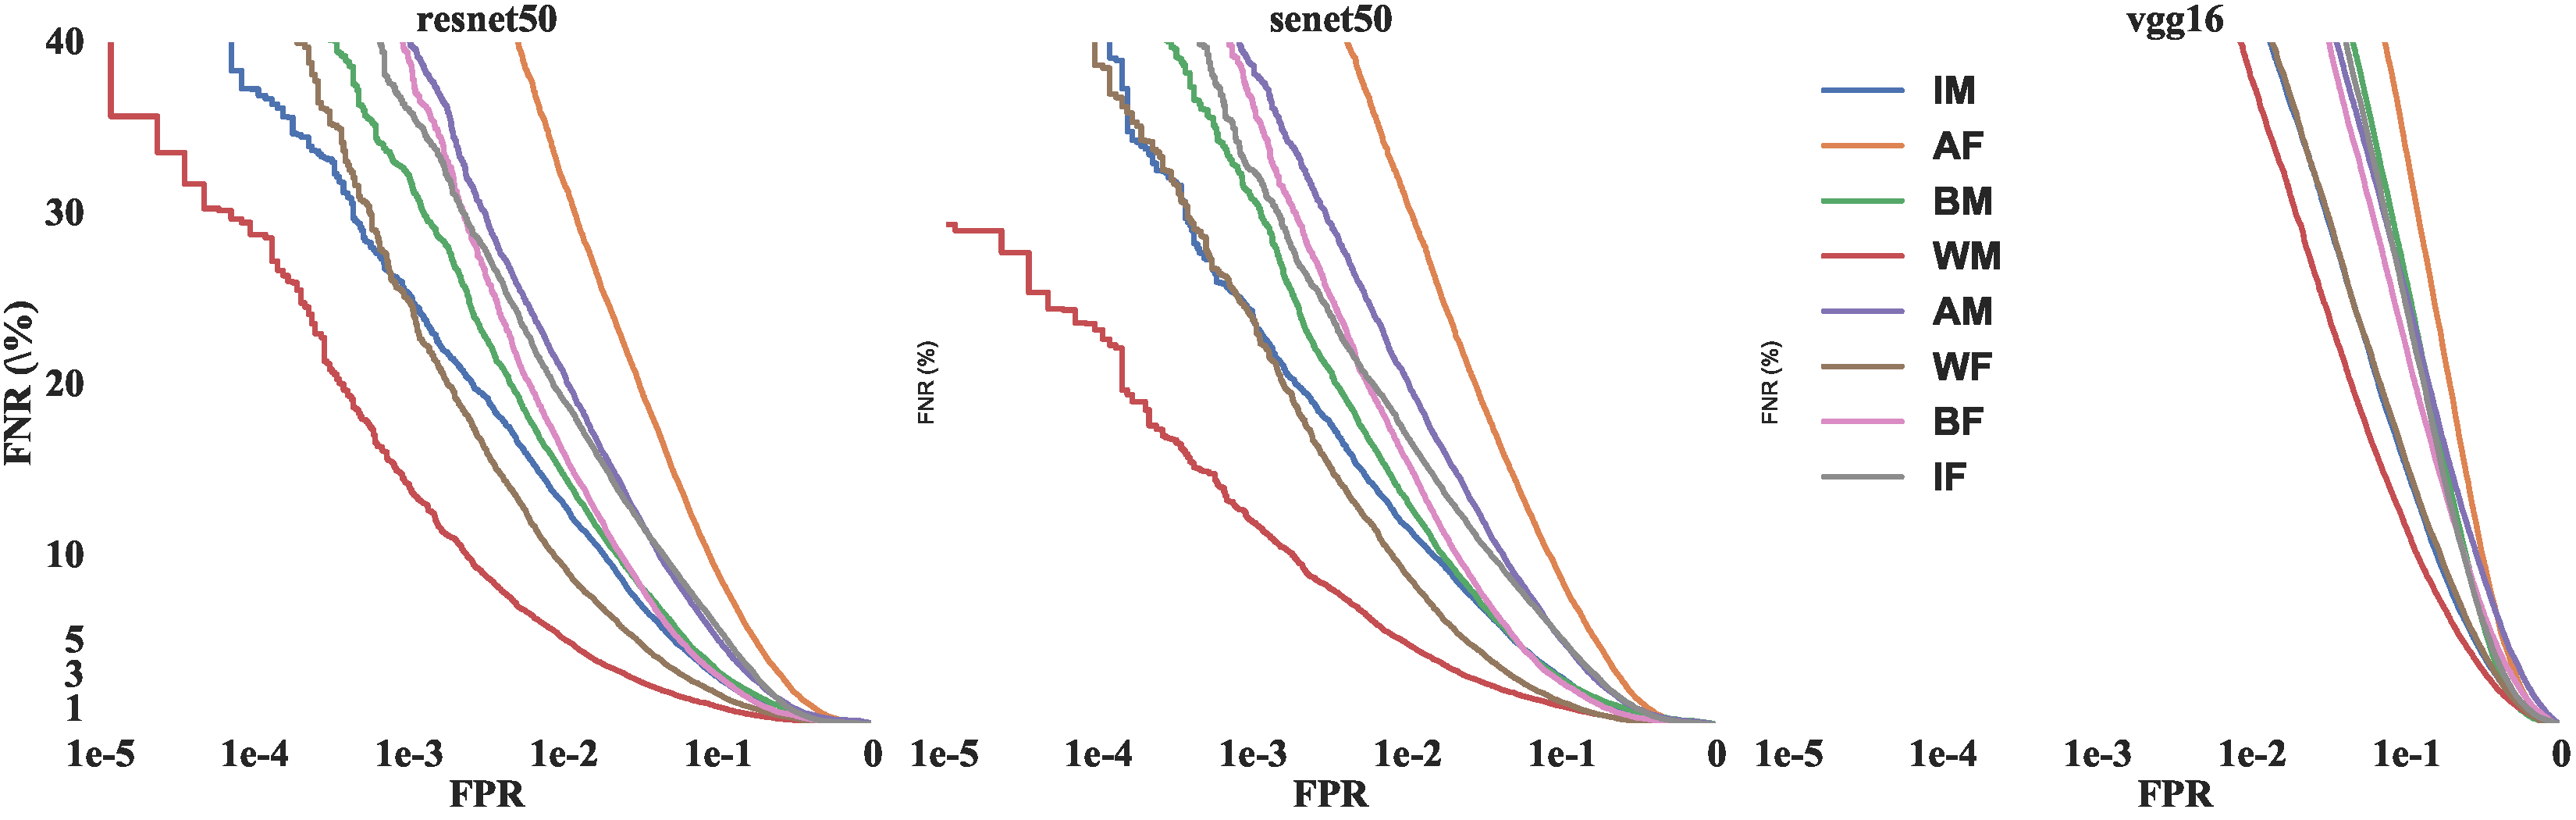
\includegraphics[width=.8\linewidth, trim={0mm 0mm 0mm 0mm},clip]{figures/SDM.pdf}\\
%     \caption{\textbf{\gls{det} curves for different CNN models}. \gls{fnr} (\%) (vertical) vs \gls{fpr} (log-scale)  (horizontal) for VGG2~\cite{Cao18} models with different backbones (vgg16, Resnet50~\cite{he2016deep}, SEnet50~\cite{hu2018squeeze}). Lower is better. For each plot, \gls{wm} is the best performing curve, \gls{af} is the worst. The the ordering of the curves is roughly the same for each backbone.}\label{fig:sdm-appendix-a}
%     \vspace{-3mm}
% \end{figure}


\begin{figure}[h!]
\vspace{-1mm}
    \centering
    \begin{subfigure}[t]{.3\linewidth}
    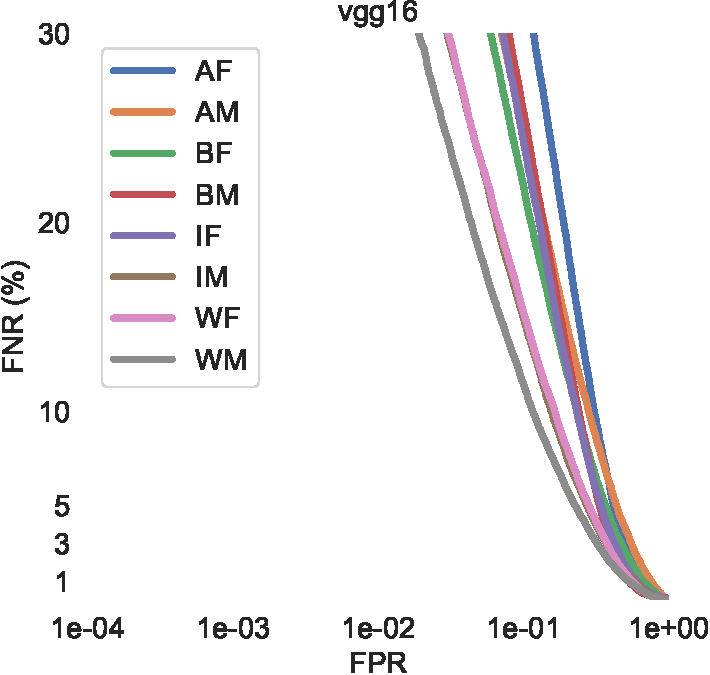
\includegraphics[width=.75\linewidth]{figures/curve_vgg16_subgroups-crop.pdf}
    \caption{VGG16~\cite{simonyan2014very}}
 \end{subfigure}
    \begin{subfigure}[t]{.27\linewidth}
    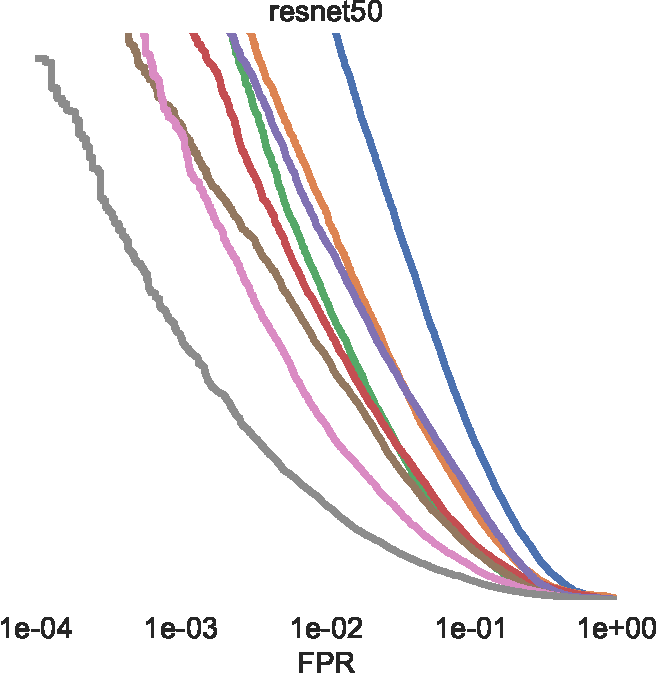
\includegraphics[width=.8\linewidth]{figures/curve_resnet50_subgroups-crop.pdf}
    \caption{ResNet50~\cite{he2016deep}}
   \end{subfigure}
    \begin{subfigure}[t]{.27\linewidth}
    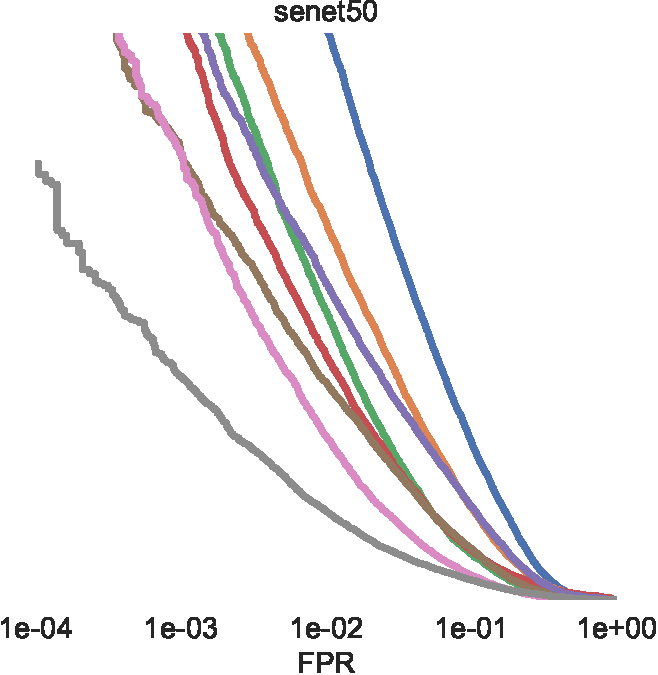
\includegraphics[width=.8\linewidth]{figures/curve_senet50_subgroups-crop.pdf}
    \caption{SENet~\cite{hu2018squeeze}}
    \end{subfigure}
    \caption{\textbf{\gls{det} curves for different CNN models}. \gls{fnr} (\%) (vertical) vs \gls{fpr} (log-scale)  (horizontal) for VGG2~\cite{Cao18} models with different backbones (VGG16, Resnet50, SEnet50). Lower is better. For each plot, \gls{wm} is the best performing curve, \gls{af} is the worst. The the ordering of the curves is roughly the same for each backbone.}\label{fig:sdm-appendix-a}
    \vspace{-1mm}
\end{figure}



Sample faces per subgroup of the \gls{bfw} dataset are shown in Fig.~\ref{fig:montage:app}.
\begin{figure}[h!]
\vspace{-2mm}
    \centering
    \includegraphics[width=.7\linewidth]{figures/facemontage.pdf}
    \caption{\textbf{Sample of \gls{bfw}}. Each row depicts a different gender, \gls{f} (top) and \gls{m} (bottom). Columns are grouped by ethnicity (\ie \gls{a}, \gls{b}, \gls{i}, and \gls{w}, respectfully).}
    \label{fig:montage:app}
    \vspace{-1mm}
\end{figure}
{
\scriptsize
\begin{thebibliography}{widest entry}
 \bibitem[1]{Cao18} Qiong Cao, Li Shen, Weidi Xie, Omkar M. Parkhi, and Andrew Zisserman. ``Vggface2: A dataset for recognising faces across pose and age.'' In \textit{IEEE International Conference on Automatic Face \& Gesture Recognition.} 2018.
 \bibitem[2]{simonyan2014very} Karen Simonyan and Andrew Zisserman. ``Very deep convolutional networks for large-scale image recognition'' \textit{arXiv preprint arXiv:1409.1556.} 2014.
  \bibitem[3]{he2016deep} He, Kaiming, Xiangyu Zhang, Shaoqing Ren, and Jian Sun. ``Deep residual learning for image recognition.'' In \textit{IEEE Conference on Computer Vision and Pattern Recognition.} 2016.
 \bibitem[4]{hu2018squeeze} Hu, Jie, Li Shen, and Gang Sun. ``Squeeze-and-excitation networks.'' In \textit{IEEE Conference on Computer Vision and Pattern Recognition.} 2018.
\end{thebibliography}
}

% \end{minipage*}
\end{bibunit}

\end{document}